% 附录 AD：边界台基与 L-H 模——约束改善从哪里来，又在哪里被限制（v1.26.8 新增）
% 数值唯一来源：tools/calc/appAD_calc.py -> tools/calc/appAD_calc.txt（正文数字的唯一来源；检查项 P36）
% 单位写法：m / s / T / Pa / A m^-2 / MW / MJ / GW m^-2，全部走 \mathrm{}，不把中文字符放进数学字体。
% 版权口径：只借鉴经典教材与文献的物理结论、定标形式与题型；文字、数值与表格自拟并独立复算。
% 本书不列 DOI，只给书名、作者、年份、卷期页。
% 分工：附录 S 讲能量约束与输运、附录 N 讲壁与偏滤器、附录 V 讲破裂、附录 X 讲辐射；
%       本附录补上一直没算完的一段——约束改善的「边界」本身：L-H 阈值、台基、ELM 与 SOL 热流。
% 声明值（定标系数、alpha_crit、材料阈值、t_ELM、tau_E、弹丸原子数等）在脚本 [DECLARED] 段逐条列出。

\section{从 L 模到 H 模：一个阈值，一次输运壁垒}
\label{sec:app-ad-threshold}
\setlength{\emergencystretch}{5em}

前面各附录一直把「约束好不好」当成一个给定的数。它有一半来自\textbf{等离子体边缘}。

同一条加热功率曲线下，托卡马克会在某一时刻突然换一种状态：边缘的湍流被压住，
密度和压强剖面在最外面十几厘米里陡起来，储能上升、约束时间提高约一倍。
这就是 L 模到 H 模的转换，1982 年在 ASDEX 上第一次被认出来。
它不是靠把某个参数调到极值，而是靠\textbf{输入功率越过一个阈值}。

阈值最先被总结成定标律。用 2008 年的多装置拟合（Martin 定标），阈值功率为

\begin{equation}
P_{\mathrm{th}}=0.0488\,n_{20}^{0.717}B^{0.803}S^{0.941}\ \mathrm{MW}
=63.2554\ \mathrm{MW},
\label{eq:app-ad-pth}
\end{equation}

其中 $n_{20}$ 是以 $10^{20}\ \mathrm{m^{-3}}$ 为单位的线平均密度，$S$ 是等离子体表面积，
工作点取 $S=489.532\ \mathrm{m^2}$（与附录 X 同一数值）、$B=5.3\ \mathrm{T}$、$n_{20}=1.0$。

工作点的 alpha 自加热是 $P_\alpha=111.3\ \mathrm{MW}$，已经是阈值的 $1.75953$ 倍；
把辅助加热和芯部辐射一起算进去，穿过分界面的功率是

\begin{equation}
P_{\mathrm{SOL}}=P_\alpha+P_{\mathrm{aux}}-P_{\mathrm{rad,core}}
=111.3+20-27.8322=103.468\ \mathrm{MW},
\qquad \frac{P_{\mathrm{SOL}}}{P_{\mathrm{th}}}=1.63572,
\label{eq:app-ad-psol}
\end{equation}

余量 $40.2124\ \mathrm{MW}$。\textbf{这个工作点不需要辅助加热就能进 H 模}：
$P_\alpha/P_{\mathrm{th}}=1.75953>1$。自加热足够撑起边缘的输运壁垒，这是点火型装置的关键性质之一。

阈值之外还有一个上限，来自密度。超过它，边缘会冷掉、辐射崩塌、约束退回 L 模：

\begin{equation}
n_G=\frac{I_p}{\pi a^2}=1.19366\times10^{20}\ \mathrm{m^{-3}},
\qquad f_G=\frac{n_e}{n_G}=0.837758,
\label{eq:app-ad-greenwald}
\end{equation}

即工作点坐在密度极限的 $84\%$ 处——这是托卡马克运行的常规区间（$0.7$--$0.9$），
再往上就要付出边缘冷却的代价。

阈值还有一个细节：回去比进来容易。H 模一旦建立，可以把功率降到 $0.65P_{\mathrm{th}}=41.116\ \mathrm{MW}$
才退回 L 模。这段回滞（hysteresis）说明壁垒不靠功率维持：
边缘剖面一旦建立，它就自己维持自己，所谓「自组织」。

阈值对参数的敏感度：密度减半，阈值降到 $38.4821\ \mathrm{MW}$；密度加倍，
阈值升到 $103.977\ \mathrm{MW}$（$\propto n^{0.717}$）。磁场从 $5.3\ \mathrm{T}$ 降到 $4\ \mathrm{T}$，
阈值降到 $50.4612\ \mathrm{MW}$；升到 $6\ \mathrm{T}$，阈值升到 $69.881\ \mathrm{MW}$（$\propto B^{0.803}$）。
\emph{低密度、高磁场}是最容易进 H 模的方向。

\begin{table}[htbp]
\centering
\small
\begin{tabular}{p{3.4cm}p{3.3cm}p{4.2cm}p{4.0cm}}
\toprule
量 & 数值 & 表达式 & 说明 \\
\midrule
L-H 阈值 & $63.2554\ \mathrm{MW}$ & $0.0488 n_{20}^{0.717}B^{0.803}S^{0.941}$ & 工作点的阈值 \\
alpha 自加热 & $111.3\ \mathrm{MW}$ & $1.75953P_{\mathrm{th}}$ & 单独就够进 H 模 \\
穿越分界面功率 & $103.468\ \mathrm{MW}$ & $P_\alpha+P_{\mathrm{aux}}-P_{\mathrm{rad,core}}$ & $=1.63572P_{\mathrm{th}}$ \\
阈值余量 & $40.2124\ \mathrm{MW}$ & $P_{\mathrm{SOL}}-P_{\mathrm{th}}$ & 可用于辐射与输运 \\
H$\to$L 反向阈值 & $41.116\ \mathrm{MW}$ & $0.65P_{\mathrm{th}}$ & 回滞宽度 \\
格林沃尔德密度 & $1.19366\times10^{20}\ \mathrm{m^{-3}}$ & $I_p/(\pi a^2)$ & $f_G=0.837758$ \\
\bottomrule
\end{tabular}
\caption{L-H 阈值与工作点。阈值是「输入打平边缘损失」的位置，不是某个可调旋钮的最佳值。}
\label{tab:app-ad-threshold}
\end{table}

那壁垒到底是什么？主流图像是\textbf{径向电场剪切}：边缘的压强梯度把离子推开，
建立径向电场 $E_r$，它产生的 $E\times B$ 流在极向把湍流涡旋撕开，
涡旋来不及长到饱和就被剪碎，于是输运系数掉下来。要压住湍流，剪切率得追上湍流的增长率。
把增长率做序估计：$\gamma\sim c_s/a$，其中离子声速

\begin{equation}
c_s=\sqrt{\frac{T_e}{m_i}}=5.93524\times10^{5}\ \mathrm{m\,s^{-1}}
=593.524\ \mathrm{km\,s^{-1}},
\qquad \gamma\sim\frac{c_s}{a}=2.96762\times10^{5}\ \mathrm{s^{-1}}.
\label{eq:app-ad-shear}
\end{equation}

要在宽度 $\Delta_{\mathrm{ped}}$ 上产生这么快的剪切，需要的极向速度与径向电场是

\begin{equation}
v_\theta\gtrsim\gamma\Delta_{\mathrm{ped}}=3.54936\times10^{4}\ \mathrm{m\,s^{-1}},
\qquad
E_r=v_\theta B_\theta\gtrsim53.2405\ \mathrm{kV\,m^{-1}},
\label{eq:app-ad-er}
\end{equation}

用的是极向磁场 $B_\theta=1.5\ \mathrm{T}$（下一节算）。作为对照，若实测 $E_r=30\ \mathrm{kV\,m^{-1}}$，
剪切率只有 $1.67220\times10^{5}\ \mathrm{s^{-1}}$，即 $\gamma$ 的 $0.563481$——
\emph{不够}。这解释了为什么 H 模总是「开关式」出现的：剪切率和湍流增长率在同一个量级上咬合，
谁稍稍占上风，结果就完全不同。

\begin{tip}{阈值不是「加热到多少」，是「输入压过损失」}{tip-app-ad-threshold}
把 L-H 阈值当成一条工程线是误读。它的物理内容是：边缘的湍流输运有一个损失率，
输入功率必须先把这部分损失打平，剩下的才能拿去建立剪切。
所以同一台装置换密度、换磁场、换尺寸，阈值都会变——定标律之所以有 $0.7$ 到 $0.9$ 次方的指数，
正是因为损失率本身随这些量变化。
\end{tip}

{\footnotesize
\textbf{出处：}L-H 转换的实验发现参照 Wagner 等（1982，\emph{Phys. Rev. Lett.} \textbf{49}, 1408）。
阈值定标的形式与指数参照 Martin、Takizuka 与 H 模数据库工作组（2008，
\emph{J. Phys. Conf. Ser.} \textbf{123}, 012033），系数 $0.0488$ 在脚本里作为声明值写出。
密度极限参照 Greenwald 等（1988，\emph{Nucl. Fusion} \textbf{28}, 2199）。
回滞与边缘剪切图像参照 Wesson \emph{Tokamaks}（第 4 版，2011，第 14 章）与
ITER Physics Basis（1999，\emph{Nucl. Fusion} \textbf{39}, 2137）。
}

\begin{figure}[htbp]
\centering
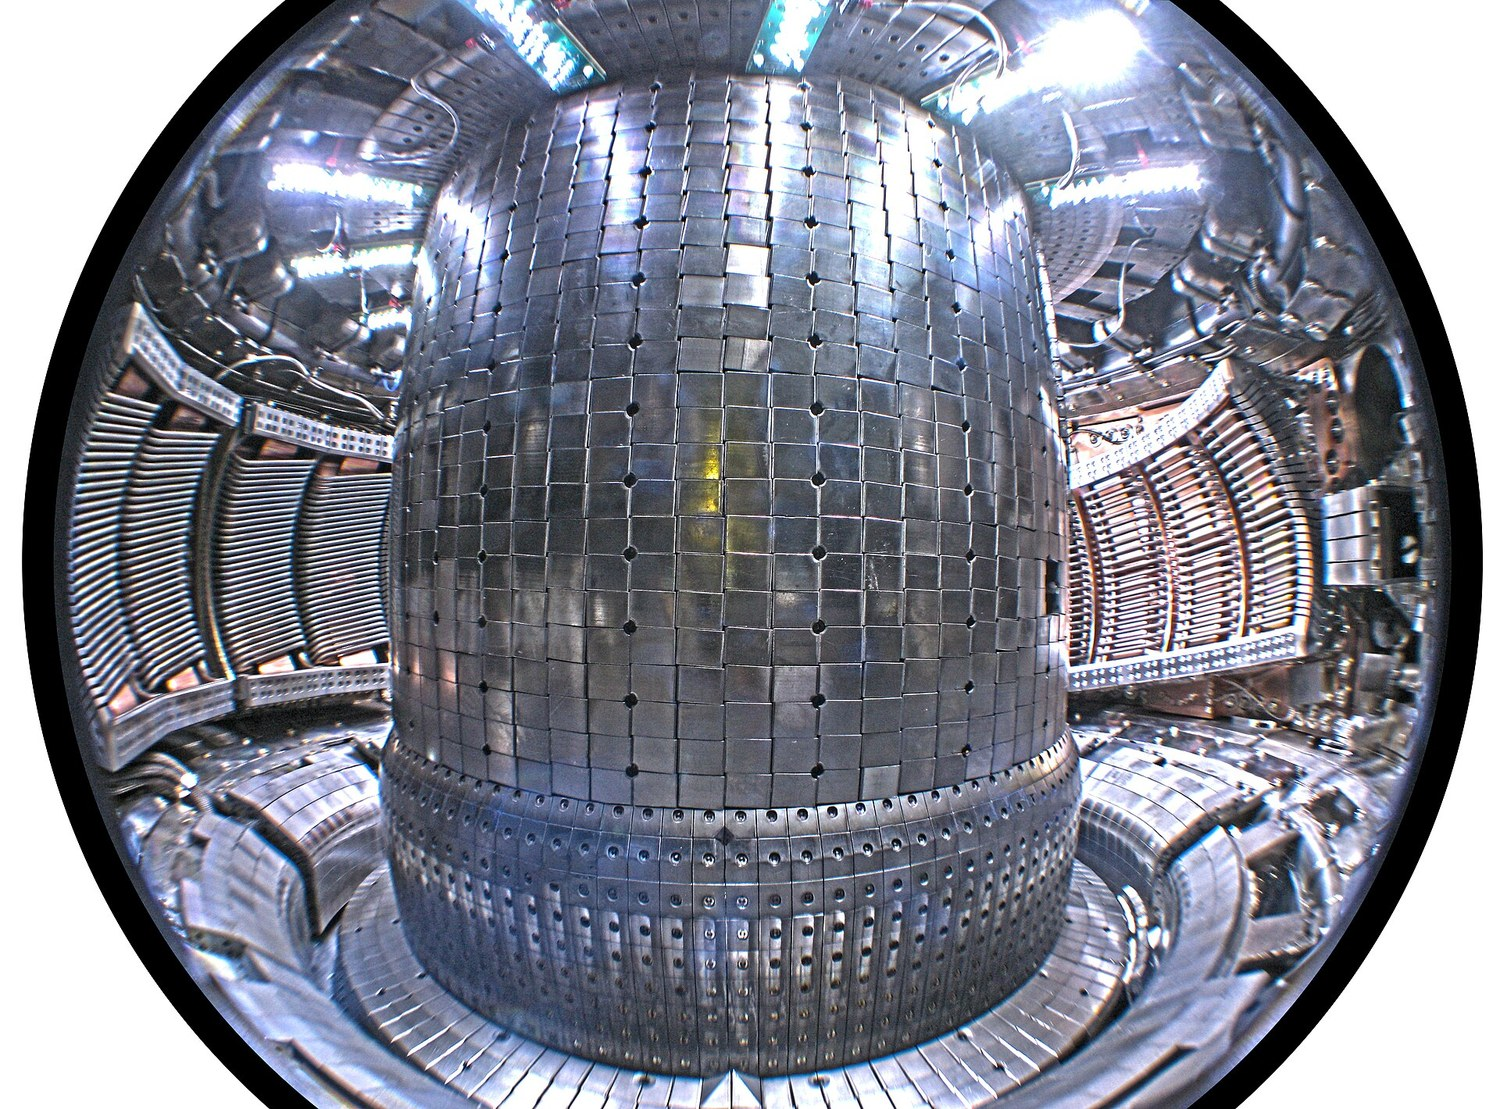
\includegraphics[width=0.72\textwidth]{../figures/ad_cmod_interior.jpg}
\caption{芯部再热，决定约束的仍是贴着壁的那一层：台基就长在这里。本节估的台基宽度、压强梯度与边界功率，说的都是图中这条内壁附近的薄层。}
\label{fig:photo-appad2}
\figsource{Mike Garrett，CC BY 3.0（Wikimedia Commons）}
\end{figure}

\begin{figure}[htbp]
\centering
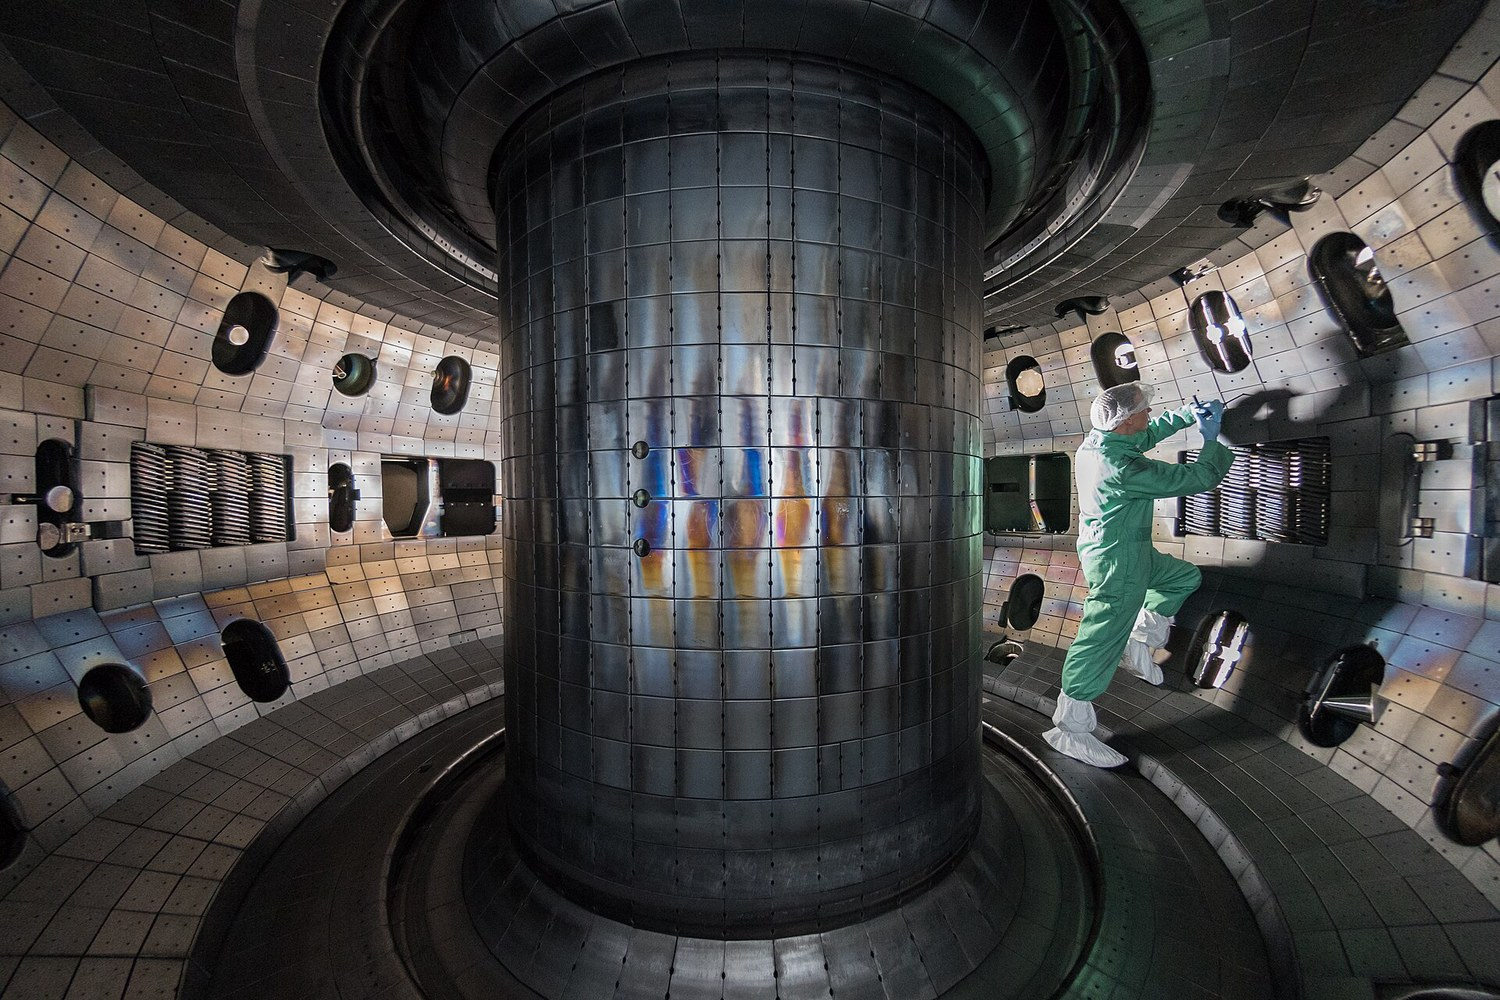
\includegraphics[width=0.78\textwidth]{../figures/ad_tocamac_chamber.jpg}
\caption{从真空室里看托卡马克：第一壁与偏滤器靶板围出的这一圈，就是台基所在的位置。台基只有十几厘米厚，却决定了一半的约束——本节算的正是这层壳的宽度与高度。}
\label{fig:photo-appad3}
\figsource{Rswilcox，CC BY-SA 4.0（Wikimedia Commons）}
\end{figure}

\section{台基：十二厘米的壳层，撑起一半约束}
\label{sec:app-ad-pedestal}

H 模的剖面在边缘多出一个「台阶」：从分界面往里，密度和温度在十几厘米内从很小抬到很高，
再往里是平缓的芯部。这个台阶叫\textbf{台基}（pedestal）。它有多高、多宽、梯度多陡，基本决定整条剖面的边界条件，也决定约束能好多少。

先算台基的宽度尺度。台基里的离子沿磁力线转圈，但「有效」的回旋半径要用极向磁场：

\begin{equation}
B_\theta=\frac{\mu_0 I_p}{2\pi a}=1.5\ \mathrm{T},
\qquad
\rho_i=\frac{\sqrt{2m_iT_i}}{eB}=4.13338\ \mathrm{mm},
\qquad
\rho_\theta=\rho_i\frac{B}{B_\theta}=1.46046\ \mathrm{cm},
\label{eq:app-ad-rhoi}
\end{equation}

取 $I_p=15\ \mathrm{MA}$、$T_i=9.194\ \mathrm{keV}$、$m_i=2.5m_p$。
$\rho_\theta$ 是有物理含义的最小宽度：台基不可能比它更窄。
湍流尺度也由它定：$k_\theta=1/\rho_i=241.933\ \mathrm{m^{-1}}$。

台基顶的压强取「密度 $0.6n_e$、温度 $3\ \mathrm{keV}$」（声明值），与体积平均压强对照：

\begin{equation}
p_{\mathrm{ped}}=2n_{\mathrm{ped}}T_{\mathrm{ped}}=57.6784\ \mathrm{kPa},
\qquad
\langle p\rangle=\frac{2W_{\mathrm{th}}}{3V}=297.525\ \mathrm{kPa},
\qquad
\frac{p_{\mathrm{ped}}}{\langle p\rangle}=0.193861,
\label{eq:app-ad-pped}
\end{equation}

即台基顶的压强约为平均压强的五分之一——边缘不算太薄。

宽度本身不是自由参数。经验定标（EPED 类）把它与台基极向 beta 绑在一起：

\begin{equation}
\beta_{p,\mathrm{ped}}=\frac{2\mu_0 p_{\mathrm{ped}}}{B_\theta^2}=0.0644273,
\qquad
\Delta_{\mathrm{ped}}=0.076\sqrt{\beta_{p,\mathrm{ped}}}\,R=11.9603\ \mathrm{cm},
\label{eq:app-ad-width}
\end{equation}

也就是 $\Delta_{\mathrm{ped}}=8.18937\,\rho_\theta$。台基总 beta 只有 $0.5161\%$，
而芯部 beta 约 $3.993\%$——\emph{边缘的 beta 很小，但梯度极大}。

把压强从台基顶降到零只用了十二厘米，于是梯度是

\begin{equation}
\left|\frac{dp}{dr}\right|=\frac{p_{\mathrm{ped}}}{\Delta_{\mathrm{ped}}}
=4.82250\times10^{5}\ \mathrm{Pa\,m^{-1}},
\qquad
\alpha_{\mathrm{MHD}}=\frac{2\mu_0Rq_{95}^2}{B^2}\left|\frac{dp}{dr}\right|=3.27709,
\label{eq:app-ad-grad}
\end{equation}

其中 $q_{95}=3.5$、$\varepsilon=a/R=0.322581$、台基顶半径 $r_{\mathrm{ped}}=a-\Delta_{\mathrm{ped}}=1.8804\ \mathrm{m}$。

台基还有一个副产品：这么陡的梯度会驱动\textbf{自举电流}。用标准形式的序估计
（系数取 $1.5$，声明值）：

\begin{equation}
j_{\mathrm{bs}}=1.5\frac{\sqrt{\varepsilon}}{B_\theta}\left|\frac{dp}{dr}\right|
=2.73900\times10^{5}\ \mathrm{A\,m^{-2}},
\qquad
\frac{j_{\mathrm{bs}}}{j_{\mathrm{avg}}}=0.229462,
\qquad
I_{\mathrm{bs}}=1.27616\ \mathrm{MA},
\label{eq:app-ad-jbs}
\end{equation}

其中 $j_{\mathrm{avg}}=I_p/(\pi a^2)=1.19366\times10^{6}\ \mathrm{A\,m^{-2}}$，
$I_{\mathrm{bs}}/I_p=0.085077$。边缘十几厘米里长出了总电流的 $8.5\%$，它正是下一节「剥离模」的驱动源。

\begin{table}[htbp]
\centering
\small
\begin{tabular}{p{3.5cm}p{3.2cm}p{4.1cm}p{4.1cm}}
\toprule
量 & 数值 & 表达式 & 说明 \\
\midrule
台基宽度 & $11.9603\ \mathrm{cm}$ & $0.076\sqrt{\beta_{p,\mathrm{ped}}}R$ & $=8.18937\rho_\theta$ \\
台基顶压强 & $57.6784\ \mathrm{kPa}$ & $2n_{\mathrm{ped}}T_{\mathrm{ped}}$ & $=0.193861\langle p\rangle$ \\
台基梯度 & $4.82250\times10^{5}\ \mathrm{Pa\,m^{-1}}$ & $p_{\mathrm{ped}}/\Delta_{\mathrm{ped}}$ & 比芯部平均陡一个量级 \\
气球参数 & $3.27709$ & $2\mu_0Rq_{95}^2|dp/dr|/B^2$ & 与判据 $2.5$--$4$ 相比 \\
自举电流密度 & $2.73900\times10^{5}\ \mathrm{A\,m^{-2}}$ & $1.5\sqrt{\varepsilon}|dp/dr|/B_\theta$ & $=0.229462j_{\mathrm{avg}}$ \\
台基自举电流 & $1.27616\ \mathrm{MA}$ & $j_{\mathrm{bs}}\Delta_{\mathrm{ped}}2\pi R$ & $=0.085077I_p$ \\
台基总 beta & $0.5161\%$ & $2\mu_0p_{\mathrm{ped}}/B^2$ & 芯部约 $3.993\%$ \\
\bottomrule
\end{tabular}
\caption{台基的几何与梯度。宽度由 beta 定，梯度由宽度定，自举电流由梯度定——一环扣一环。}
\label{tab:app-ad-pedestal}
\end{table}

\begin{tip}{台基宽度不是自由参数}{tip-app-ad-width}
很多剖面拟合把台基宽度当成可调参数。但物理上它与台基极向 beta 挂钩：
想把台基压强做高，宽度会自己变化，梯度随之变化，最后又回到稳定性边界上。
\emph{能独立调节的只有台基顶压强和宽度这两个量中的一个}，另一个由稳定性决定。
\end{tip}

{\footnotesize
\textbf{出处：}台基宽度与高度的经验定标参照 Snyder 等（2011，\emph{Nucl. Fusion} \textbf{51}, 103008）
与 Snyder 等（2002，\emph{Phys. Plasmas} \textbf{9}, 2037）。
极向回旋半径作为最小宽度尺度的论证参照
Connor、Hastie 与 Taylor（1978，\emph{Phys. Rev. Lett.} \textbf{40}, 396）。
自举电流的标准形式参照 Wesson \emph{Tokamaks}（第 4 版，2011，第 4 章），
序系数 $1.5$ 与 $0.076$ 一样是声明值。
}

\section{两条边界的夹缝：气球模与剥离模}
\label{sec:app-ad-limits}

台基梯度陡、边缘电流又大，于是有两条独立的稳定性边界同时压着它。

第一条是\textbf{气球模}（ballooning）：磁力线在坏曲率区被压强梯度推着往外鼓。
把判据写成压强上限，宽度就出现在分子上：

\begin{equation}
p_{\max}=\frac{\alpha_{\mathrm{crit}}B^2}{2\mu_0Rq_{95}^2}\Delta_{\mathrm{ped}}
=\begin{cases}
44.0012\ \mathrm{kPa}, & \alpha_{\mathrm{crit}}=2.5\ \text{（无自举）},\\
70.4019\ \mathrm{kPa}, & \alpha_{\mathrm{crit}}=4.0\ \text{（含自举）}.
\end{cases}
\label{eq:app-ad-pmax}
\end{equation}

工作点声明的台基压强是 $57.6784\ \mathrm{kPa}$，夹在这两个数中间。

\begin{equation}
\frac{\alpha_{\mathrm{MHD}}}{\alpha_{\mathrm{crit}}}
=\begin{cases}
1.31084, & \text{无自举判据},\\
0.819273, & \text{含自举判据}.
\end{cases}
\label{eq:app-ad-margin}
\end{equation}

第二条是\textbf{剥离模}（peeling）：边缘的自举电流密度已经达到平均电流密度的 $0.229462$、
总电流的 $0.085077$，它自身的电流梯度会驱动一种类似扭曲模的不稳定性。两条边界在
$(\alpha,\ j_{\mathrm{edge}})$ 平面上围出一个「鼻子」形的稳定区，台基就坐在这个鼻子的尖端附近。

台基壳层自身的储能并不大：

\begin{equation}
\begin{aligned}
V_{\mathrm{ped}}&=S\Delta_{\mathrm{ped}}=58.5493\ \mathrm{m^3}=7.03548\%\,V,\\
W_{\mathrm{ped}}&=\frac{3}{2}\cdot\frac{p_{\mathrm{ped}}}{2}V_{\mathrm{ped}}
=2.53277\ \mathrm{MJ}=0.00681952\,W_{\mathrm{th}}.
\end{aligned}
\label{eq:app-ad-wped}
\end{equation}

台基壳层里的储能连总储能的 $1\%$ 都不到，可它一旦坍塌，
损失的能量却是总储能的百分之几（下一节）。\emph{坍塌波及的范围比台基壳层深}，
这是理解 ELM 的第一件事。

\begin{table}[htbp]
\centering
\small
\begin{tabular}{p{3.6cm}p{3.2cm}p{3.9cm}p{4.2cm}}
\toprule
量 & 数值 & 表达式 & 说明 \\
\midrule
气球模上限（无自举） & $44.0012\ \mathrm{kPa}$ & $\alpha_{\mathrm{crit}}B^2\Delta/2\mu_0Rq_{95}^2$ & $\alpha_{\mathrm{crit}}=2.5$ \\
气球模上限（含自举） & $70.4019\ \mathrm{kPa}$ & 同上 & $\alpha_{\mathrm{crit}}=4.0$ \\
工作点台基压强 & $57.6784\ \mathrm{kPa}$ & $2n_{\mathrm{ped}}T_{\mathrm{ped}}$ & 落在两条判据之间 \\
比值 & $1.31084$ / $0.819273$ & $\alpha_{\mathrm{MHD}}/\alpha_{\mathrm{crit}}$ & 与判据同量级 \\
边缘电流分数 & $0.229462$ & $j_{\mathrm{bs}}/j_{\mathrm{avg}}$ & 剥离模驱动源 \\
台基壳层体积 & $58.5493\ \mathrm{m^3}$ & $S\Delta_{\mathrm{ped}}$ & $=7.03548\%\,V$ \\
壳层储能 & $2.53277\ \mathrm{MJ}$ & $3p_{\mathrm{ped}}V_{\mathrm{ped}}/4$ & $<1\%\,W_{\mathrm{th}}$ \\
\bottomrule
\end{tabular}
\caption{两条稳定性边界。台基之所以「刚好」存在，是因为再高一点就会被模吃掉。}
\label{tab:app-ad-limits}
\end{table}

\begin{tip}{台基不是「越高越好」}{tip-app-ad-two-branches}
压强越高，约束越好——这话对芯部成立，对边缘不成立。边缘的压强梯度每提高一点，
气球模和剥离模的驱动力就各涨一点，直到越界。H 模之所以能稳定存在，靠的是把工作点停在稳定区鼻尖附近，再用旋转与剪切压住剩余的增长。
\end{tip}

{\footnotesize
\textbf{出处：}理想气球模判据的 $\alpha$ 参数与临界值参照 Connor、Hastie 与 Taylor
（1978，\emph{Phys. Rev. Lett.} \textbf{40}, 396）。
剥离-气球模稳定区与「鼻子」形边界参照
Snyder 等（2002，\emph{Phys. Plasmas} \textbf{9}, 2037）。
气球模与剥离模的导出过程
参照 Freidberg \emph{Ideal MHD}（2014，第 8、11 章）。本附录只借判据形式，
$\alpha_{\mathrm{crit}}$ 的两个取值作为声明值写在脚本里。
}

\section{ELM：储能的周期性坍塌}
\label{sec:app-ad-elm}

台基把压强堆到边界附近，但它不能一直堆着：边缘的压强梯度一旦越界，
一次\textbf{边缘局域模}（ELM）爆发，把台基在几百微秒内削掉一层，然后重新长起来。
H 模的常态就是「堆积—坍塌」的循环。

先算一次坍塌要带走多少能量。取类型 I ELM 的常规值 $\Delta W_{\mathrm{ELM}}=0.07W_{\mathrm{th}}$：

\begin{equation}
\Delta W_{\mathrm{ELM}}=0.07\,W_{\mathrm{th}}=2.59980\times10^{7}\ \mathrm{J}=25.998\ \mathrm{MJ}.
\label{eq:app-ad-dwelm}
\end{equation}

这些能量最终落在偏滤器上。偏滤器的能量沉积面积取极向长度 $L_{\mathrm{div}}=1\ \mathrm{m}$ 的环带，
$A_{\mathrm{div}}=2\pi RL_{\mathrm{div}}=38.9557\ \mathrm{m^2}$，于是

\begin{equation}
\begin{aligned}
\frac{\Delta W_{\mathrm{ELM}}}{A_{\mathrm{div}}}&=6.67373\times10^{5}\ \mathrm{J\,m^{-2}}
=0.667373\ \mathrm{MJ\,m^{-2}},\\
q_{\mathrm{ELM}}&=\frac{0.667373\ \mathrm{MJ\,m^{-2}}}{0.3\ \mathrm{ms}}
=2.22458\ \mathrm{GW\,m^{-2}},
\end{aligned}
\label{eq:app-ad-eden}
\end{equation}

上升时间取 $t_{\mathrm{ELM}}=0.3\ \mathrm{ms}$（声明值）。钨靶板的能量密度阈值按 $1\ \mathrm{MJ\,m^{-2}}$
估计，那么这一次 ELM 用掉了阈值的 $0.667373$，余量只有 $1.49841$ 倍——
\emph{一次大 ELM 就够把安全余量吃掉三分之二}。

ELM 的频率不是可以从外面随便拧的旋钮，它由功率平衡定：稳态下，
ELM 通道带走的时间平均功率必须等于输入功率，

\begin{equation}
f_{\mathrm{ELM}}=\frac{P_{\mathrm{SOL}}}{\Delta W_{\mathrm{ELM}}}
=\frac{103.468\ \mathrm{MW}}{25.998\ \mathrm{MJ}}=3.97984\ \mathrm{Hz},
\qquad
T_{\mathrm{ELM}}=\frac{1}{f_{\mathrm{ELM}}}=251.267\ \mathrm{ms}.
\label{eq:app-ad-felm}
\end{equation}

自洽性检查：$f_{\mathrm{ELM}}\Delta W_{\mathrm{ELM}}=103.468\ \mathrm{MW}=P_{\mathrm{SOL}}$。
与能量约束时间对照，$f_{\mathrm{ELM}}\tau_E=14.7254$：每个约束时间里发生约 $15$ 次坍塌，
而台基壳层自身的恢复功率只有 $W_{\mathrm{ped}}/\tau_E=0.684532\ \mathrm{MW}$——
\emph{坍塌带走的能量远多于台基壳层里存的那点}，ELM 的扰动深度比台基宽度大。

\begin{table}[htbp]
\centering
\small
\begin{tabular}{p{3.6cm}p{3.3cm}p{4.0cm}p{4.0cm}}
\toprule
量 & 数值 & 表达式 & 说明 \\
\midrule
单次 ELM 损失 & $25.998\ \mathrm{MJ}$ & $0.07W_{\mathrm{th}}$ & 类型 I 常规值 \\
偏滤器面积 & $38.9557\ \mathrm{m^2}$ & $2\pi RL_{\mathrm{div}}$ & $L_{\mathrm{div}}=1\ \mathrm{m}$ \\
能量密度 & $0.667373\ \mathrm{MJ\,m^{-2}}$ & $\Delta W/A_{\mathrm{div}}$ & 阈值的 $0.667373$ \\
峰值热流 & $2.22458\ \mathrm{GW\,m^{-2}}$ & $E/t_{\mathrm{ELM}}$ & $t_{\mathrm{ELM}}=0.3\ \mathrm{ms}$ \\
ELM 频率 & $3.97984\ \mathrm{Hz}$ & $P_{\mathrm{SOL}}/\Delta W_{\mathrm{ELM}}$ & 由功率平衡定 \\
ELM 周期 & $251.267\ \mathrm{ms}$ & $1/f_{\mathrm{ELM}}$ & $f_{\mathrm{ELM}}\tau_E=14.7254$ \\
\bottomrule
\end{tabular}
\caption{ELM 的能量账。频率不是自由参数，而是「输入功率要被 ELM 通道带走」的结果。}
\label{tab:app-ad-elm}
\end{table}

\begin{tip}{ELM 频率不是外部旋钮}{tip-app-ad-elm-power}
实验上观察到「加料后 ELM 变快」，常被解释成加料改变了稳定性。
更基本的解释是功率账：加料把边缘冷却、$P_{\mathrm{SOL}}$ 的分配变了，
或者把台基恢复得更快，于是同样的损失能量对应更高的频率。
想把频率当成控制量，前提是先承认它是被动的。
\end{tip}

{\footnotesize
\textbf{出处：}ELM 的分类与物理图像参照 Zohm（1996，\emph{Plasma Phys. Control. Fusion}
\textbf{38}, 105）。
类型 I ELM 的能量损失份额与上升时间量级参照 Loarte 等（2003，
\emph{Plasma Phys. Control. Fusion} \textbf{45}, 1549）。
偏滤器能量沉积与靶板阈值的处理
参照 Leonard（2014，\emph{Phys. Plasmas} \textbf{21}, 090501）与附录 N 的同一口径。
}

\section{缓解：把一次大坍塌拆成很多次小坍塌}
\label{sec:app-ad-mitigation}

既然 ELM 的能量密度离材料阈值只差 $1.5$ 倍，工程上的做法是把它\textbf{拆小、拆多}：
让同样的时间平均功率由更多次、每次更小的坍塌带走。
弹丸步调（pellet pacing）与共振磁扰动（RMP）走的是同一条逻辑。

先看弹丸步调。若用弹丸每 $50\ \mathrm{ms}$ 强制触发一次 ELM（$f=20\ \mathrm{Hz}$），
由功率平衡，每次损失的能量降到

\begin{equation}
\begin{aligned}
\Delta W&=\frac{P_{\mathrm{SOL}}}{f}=\frac{103.468\ \mathrm{MW}}{20\ \mathrm{Hz}}
=5.17339\ \mathrm{MJ},\\
\frac{\Delta W}{A_{\mathrm{div}}}&=0.132802\ \mathrm{MJ\,m^{-2}},\\
q&=\frac{0.132802\ \mathrm{MJ\,m^{-2}}}{0.3\ \mathrm{ms}}=0.442672\ \mathrm{GW\,m^{-2}},
\end{aligned}
\label{eq:app-ad-pace}
\end{equation}

能量密度降到未缓解时的 $0.199$ 倍，峰值热流从 $2.2\ \mathrm{GW\,m^{-2}}$ 掉到 $0.44\ \mathrm{GW\,m^{-2}}$。
反过来问：要把能量密度压到 $0.3\ \mathrm{MJ\,m^{-2}}$ 以下，频率至少要

\begin{equation}
f\ge\frac{P_{\mathrm{SOL}}}{0.3\ \mathrm{MJ\,m^{-2}}\cdot A_{\mathrm{div}}}
=8.85345\ \mathrm{Hz},
\label{eq:app-ad-fmin}
\end{equation}

即每 $113\ \mathrm{ms}$ 一次——这个数就是步调系统的工作点。

第二条路线是 RMP：用外部线圈在边缘加上一个与等离子体共振的静态扰动场，
把边缘的输运「打毛」，让台基始终到不了边界，于是不再有大 ELM。
共振面位置由 $q$ 剖面定（取 $q(r)=q_0+(q_{95}-q_0)(r/a)^2$，$q_0=1.0$）：

\begin{equation}
\begin{aligned}
\frac{r_n}{a}&=\sqrt{\frac{n-q_0}{q_{95}-q_0}},\\
n=3:\ r_3&=1.78885\ \mathrm{m}\ (\text{台基顶内}\ 9.15431\ \mathrm{cm}),\\
n=2:\ r_2&=1.26491\ \mathrm{m}.
\end{aligned}
\label{eq:app-ad-rmp}
\end{equation}

$n=3$ 的共振面正好落在台基底下几厘米处，所以 $n=3$ 的 RMP 能直接作用在台基上。
$n=2$ 的共振面在更里面，扰动要穿过台基才能到达，效果和代价都不同。

弹丸本身也要算：一个含 $10^{21}$ 个原子的弹丸，质量只有

\begin{equation}
m_{\mathrm{pel}}=10^{21}\times2.5m_p=4.18155\times10^{-6}\ \mathrm{kg}=4.18155\ \mathrm{mg},
\label{eq:app-ad-pellet}
\end{equation}

若全部沉积在台基壳层里，密度扰动是 $\Delta n=1.70796\times10^{19}\ \mathrm{m^{-3}}$，
相当于 $n_{\mathrm{ped}}$ 的 $28.4661\%$——足以把台基推到边界上，强制放一次小 ELM。

\begin{table}[htbp]
\centering
\small
\begin{tabular}{p{3.5cm}p{3.2cm}p{4.1cm}p{4.1cm}}
\toprule
量 & 数值 & 表达式 & 说明 \\
\midrule
步调 $20\ \mathrm{Hz}$ 的单次损失 & $5.17339\ \mathrm{MJ}$ & $P_{\mathrm{SOL}}/f$ & 未缓解的 $0.199$ 倍 \\
对应能量密度 & $0.132802\ \mathrm{MJ\,m^{-2}}$ & $\Delta W/A_{\mathrm{div}}$ & 远低于 $1\ \mathrm{MJ\,m^{-2}}$ \\
对应峰值热流 & $0.442672\ \mathrm{GW\,m^{-2}}$ & $E/t_{\mathrm{ELM}}$ & 未缓解的 $0.199$ 倍 \\
能量密度达标频率 & $8.85345\ \mathrm{Hz}$ & $P_{\mathrm{SOL}}/(0.3\,\mathrm{MJ\,m^{-2}}A_{\mathrm{div}})$ & 步调系统工作点 \\
$n=3$ RMP 共振面 & $1.78885\ \mathrm{m}$ & $a\sqrt{(3-q_0)/(q_{95}-q_0)}$ & 台基顶内 $9.15431\ \mathrm{cm}$ \\
$n=2$ RMP 共振面 & $1.26491\ \mathrm{m}$ & 同上 & 在台基以里 \\
弹丸质量 & $4.18155\ \mathrm{mg}$ & $10^{21}\times2.5m_p$ & $\Delta n=28.4661\%n_{\mathrm{ped}}$ \\
\bottomrule
\end{tabular}
\caption{两条缓解路线。目标不是「没有 ELM」，而是让每次 ELM 都落在材料阈值之下。}
\label{tab:app-ad-mitigation}
\end{table}

\begin{tip}{缓解不是消除}{tip-app-ad-mitigation}
「消掉 ELM」听起来更彻底，但代价是边缘的粒子与杂质排出通道被一起堵上——
密度会爬升、杂质会积累。RMP 抑制下常见的是「无大 ELM 但有连续小坍塌」的状态。
工程上追求的是\textbf{把不可控的大事件换成可控的小事件}，而不是把事件清零。
\end{tip}

{\footnotesize
\textbf{出处：}RMP 抑制 ELM 的实验结果参照 Evans 等（2006，\emph{Nature Physics} \textbf{2}, 419）
与 Liang 等（2007，\emph{Phys. Rev. Lett.} \textbf{98}, 265004）。
弹丸步调参照
Lang 等（2003，\emph{Nucl. Fusion} \textbf{43}, 1110）。
台基排出与密度控制的取舍
参照 Leonard（2014，\emph{Phys. Plasmas} \textbf{21}, 090501）。
}

\section{从台基到靶板：热流落在多小的地方}
\label{sec:app-ad-sol}

台基决定了「有多少热要排出去」，而真要命的是「这些热落在一个多小的面积上」。
中间隔着刮削层（SOL）：磁力线把热量沿着一个薄薄的通道导到偏滤器靶板，
通道的宽度叫\textbf{热流宽度} $\lambda_q$。

取外中平面极向磁场 $B_\theta=0.089\ \mathrm{m}$（这里用的是 $\lambda_q$ 经验定标里
$B_\theta$ 以特斯拉为单位、写成 $0.089$ 的值；它由 $B_p=\mu_0I_p/(2\pi a)$ 折算而来，
标度是 $B_\theta^{-1.19}$），则

\begin{equation}
\begin{aligned}
\lambda_q&=0.63\,B_\theta^{-1.19}=0.388859\ \mathrm{mm},\\
\lambda_t&=5\lambda_q=1.94429\ \mathrm{mm},\\
A_{\mathrm{out}}&=2\pi R\,\lambda_t\times5=0.0757414\ \mathrm{m^2}.
\end{aligned}
\label{eq:app-ad-lamq}
\end{equation}

$\lambda_q$ 只有零点几毫米——比台基宽度（$1.2\ \mathrm{cm}$）小一个数量级以上。
于是同样的 $P_{\mathrm{SOL}}$ 落在一个极小的面积上：

\begin{equation}
q_{\mathrm{peak}}=\frac{0.7\,P_{\mathrm{SOL}}}{A_{\mathrm{out}}}
=\frac{0.7\times103.468\ \mathrm{MW}}{0.0757414\ \mathrm{m^2}}
=956.246\ \mathrm{MW\,m^{-2}},
\qquad
\frac{q_{\mathrm{peak}}}{10\ \mathrm{MW\,m^{-2}}}=95.6246 .
\label{eq:app-ad-qpeak}
\end{equation}

峰值热流比材料能承受的 $10\ \mathrm{MW\,m^{-2}}$ 高\textbf{近一百倍}。要让靶板活下来，必须在热流到达之前把它「化掉」：
要么把 $\lambda_q$ 展宽，要么让能量以辐射的形式在到达靶板前就放掉（脱靶）。

先看「需要辐射掉多少」：若完全不展宽，要满足 $q_{\mathrm{peak}}\le10\ \mathrm{MW\,m^{-2}}$，
必须辐射掉

\begin{equation}
f_{\mathrm{rad}}=1-\frac{10\ \mathrm{MW\,m^{-2}}}{956.246\ \mathrm{MW\,m^{-2}}}
=0.989542,
\label{eq:app-ad-detach}
\end{equation}

即 $98.95\%$ 的 $P_{\mathrm{SOL}}$ 都要在 SOL 里以辐射形式放掉——这是「完全脱靶」的口径。
工程上更常见的组合是「适度展宽 + 部分辐射」：把 $\lambda_q$ 展宽 $5$ 倍、再辐射掉 $90\%$，
峰值热流降到

\begin{equation}
q_{\mathrm{peak}}'=\frac{0.7\,P_{\mathrm{SOL}}\times0.10}
{2\pi R\,(5\lambda_t)\times5}=19.1249\ \mathrm{MW\,m^{-2}},
\label{eq:app-ad-broaden}
\end{equation}

还不够；展宽 $5$ 倍 + 辐射 $95\%$，或展宽 $10$ 倍 + 辐射 $90\%$，才刚好到

\begin{equation}
q_{\mathrm{peak}}''=\frac{0.7\,P_{\mathrm{SOL}}\times0.05}{2\pi R\,(5\lambda_t)\times5}
=9.56246\ \mathrm{MW\,m^{-2}}\approx10\ \mathrm{MW\,m^{-2}} .
\label{eq:app-ad-broaden2}
\end{equation}

偏滤器设计因此是「辐射 + 几何」的联合优化，而不是把靶板做得更耐烧。

最后做一个对照：附录 X 算出的壁面轫致辐射热流是 $55.1547\ \mathrm{kW\,m^{-2}}$，
它与 SOL 峰值热流之比是

\begin{equation}
\frac{q_{\mathrm{peak}}}{q_{\mathrm{brems}}^{\mathrm{wall}}}
=\frac{956.246\ \mathrm{MW\,m^{-2}}}{0.0551547\ \mathrm{MW\,m^{-2}}}=17337.5 .
\label{eq:app-ad-ratio}
\end{equation}

体辐射（韧致）均匀落在整个壁上，SOL 热流沿磁力线集中到靶板——差四个数量级。

\begin{table}[htbp]
\centering
\small
\begin{tabular}{p{3.6cm}p{3.2cm}p{4.0cm}p{4.0cm}}
\toprule
量 & 数值 & 表达式 & 说明 \\
\midrule
热流宽度 & $0.388859\ \mathrm{mm}$ & $0.63B_\theta^{-1.19}$ & $B_\theta=0.089$ \\
总宽度 & $1.94429\ \mathrm{mm}$ & $5\lambda_q$ & 覆盖约 $99\%$ 热流 \\
沉积面积 & $0.0757414\ \mathrm{m^2}$ & $2\pi R\lambda_t\times5$ & 倾角因子 $5$ \\
峰值热流 & $956.246\ \mathrm{MW\,m^{-2}}$ & $0.7P_{\mathrm{SOL}}/A_{\mathrm{out}}$ & 阈值的 $95.6246$ 倍 \\
需辐射掉的比例 & $0.989542$ & $1-10/q_{\mathrm{peak}}$ & 完全不展宽 \\
展宽 $5$ 倍 + 辐射 $90\%$ & $19.1249\ \mathrm{MW\,m^{-2}}$ & 见式 & 仍超阈值 \\
展宽 $5$ 倍 + 辐射 $95\%$ & $9.56246\ \mathrm{MW\,m^{-2}}$ & 见式 & 刚好达标 \\
与壁面韧致之比 & $17337.5$ & $q_{\mathrm{peak}}/q_{\mathrm{brems}}$ & 四个数量级 \\
\bottomrule
\end{tabular}
\caption{从台基到靶板的热流账。偏滤器的存在理由就写在这一行比值里。}
\label{tab:app-ad-sol}
\end{table}

\begin{tip}{台基决定「有多少」，SOL 决定「多小」}{tip-app-ad-sol}
初学者常把「$P_{\mathrm{SOL}}$ 太大」当成偏滤器的唯一问题。其实 $P_{\mathrm{SOL}}$ 只是分子，
$\lambda_q$ 才是分母，而且 $\lambda_q$ 对 $B_\theta$、对 SOL 中的湍流输运都很敏感。
同一台装置，改变边缘的输运就能让峰值热流变化数倍——这比改材料容易得多。
\end{tip}

{\footnotesize
\textbf{出处：}热流宽度的经验定标参照 Eich 等（2013，\emph{Nucl. Fusion} \textbf{53}, 093031）
的 $\lambda_q\propto B_\theta^{-1.19}$ 形式。
偏滤器热流与脱靶的工程处理参照
Leonard（2014，\emph{Phys. Plasmas} \textbf{21}, 090501）与附录 N 的同一口径。
壁面轫致辐射热流取附录 X 的 $55.1547\ \mathrm{kW\,m^{-2}}$（同一工作点）。
}

\section{估算练习}
\label{sec:app-ad-problems}

六道题都用本附录的工作点，除题目另给条件外，其余量保持不变。

\textbf{练习 1} 若一次 ELM 带走 $0.10W_{\mathrm{th}}$（而不是 $0.07W_{\mathrm{th}}$），
能量密度是多少？还能满足 $1\ \mathrm{MJ\,m^{-2}}$ 的阈值吗？

\textbf{练习 2} 若把 $P_{\mathrm{SOL}}$ 提高到 $150\ \mathrm{MW}$，而每次 ELM 仍带走
$25.998\ \mathrm{MJ}$，ELM 频率变为多少？与工作点的 $3.97984\ \mathrm{Hz}$ 相比是几倍？

\textbf{练习 3} 一个含 $2\times10^{21}$ 个原子的弹丸（取 $m_i=2.5m_p$），
质量是多少毫克？全部沉积在台基壳层里时，密度扰动是 $n_{\mathrm{ped}}$ 的百分之多少？

\textbf{练习 4} 若 $q_{95}$ 降到 $6.5$，$n=3$ 的 RMP 共振面移到哪里？它还落在台基里吗
（台基区间 $[1.78885,\ 1.88311]\ \mathrm{m}$）？

\textbf{练习 5} 若把 $\lambda_q$ 展宽 $2$ 倍（面积翻倍），峰值热流变为多少？
此时要压到 $10\ \mathrm{MW\,m^{-2}}$ 需要辐射掉多少比例？

\textbf{练习 6} 若 $\tau_E=0.15\ \mathrm{s}$ 而 $P_{\mathrm{SOL}}$ 占 $P_{\mathrm{loss}}$ 的 $30\%$，
$P_{\mathrm{SOL}}$ 是多少？与工作点相比是几倍？峰值热流按线性外推是多少？

\textbf{解答 1} $\Delta W=0.10\times371.4\ \mathrm{MJ}=37.14\ \mathrm{MJ}$，
除以 $A_{\mathrm{div}}=38.9557\ \mathrm{m^2}$ 得 $0.953391\ \mathrm{MJ\,m^{-2}}$，
是阈值的 $0.953391$——\emph{刚刚卡在阈值以内}，余量约 $1.4$ 倍。

\textbf{解答 2} $f_{\mathrm{ELM}}=150\ \mathrm{MW}/25.998\ \mathrm{MJ}=5.76967\ \mathrm{Hz}$，
对应周期 $173.32\ \mathrm{ms}$，是工作点的 $1.44972$ 倍（与功率之比 $1.44972$ 一致——
因为 $\Delta W$ 没变）。

\textbf{解答 3} $m=2\times10^{21}\times2.5m_p=8.36311\times10^{-6}\ \mathrm{kg}=8.36311\ \mathrm{mg}$；
$\Delta n=2\times10^{21}/V_{\mathrm{ped}}=3.41592\times10^{19}\ \mathrm{m^{-3}}
=56.9321\%\,n_{\mathrm{ped}}$。这么大的扰动足以强制放一次 ELM。

\textbf{解答 4} $r_3/a=\sqrt{(3-1)/(6.5-1)}=0.603023$，$r_3=1.20605\ \mathrm{m}$，
距台基顶还有 $67.7065\ \mathrm{cm}$——\emph{已经不在台基里了}。
$q_{95}$ 越高，同样的 $n=3$ 共振面越靠里，RMP 对台基的作用越弱。

\textbf{解答 5} 面积翻倍后 $q_{\mathrm{peak}}=0.7\times103.468\ \mathrm{MW}
/0.151483\ \mathrm{m^2}=478.124\ \mathrm{MW\,m^{-2}}$，
是 $10\ \mathrm{MW\,m^{-2}}$ 的 $47.8124$ 倍；需要辐射掉 $1-10/478.124=0.979085$。
展宽把需要辐射的比例从 $0.989542$ 降到 $0.979085$——只降了一个百分点，
\emph{单靠展宽远远不够，必须配合辐射}。

\textbf{解答 6} $P_{\mathrm{loss}}=W_{\mathrm{th}}/\tau_E=371.4\ \mathrm{MJ}/0.15\ \mathrm{s}
=2.476\ \mathrm{GW}$，$P_{\mathrm{SOL}}=0.30\times2.476\ \mathrm{GW}=742.8\ \mathrm{MW}$，
是工作点的 $7.17903$ 倍。若 ELM 损失不变，$f_{\mathrm{ELM}}=28.5714\ \mathrm{Hz}$；
峰值热流按线性外推 $q_{\mathrm{peak}}=6864.94\ \mathrm{MW\,m^{-2}}$——
比工作点高 $7$ 倍多，靶板必死。\emph{约束变差时最先出问题的不是芯部，是靶板}。

\section{来源、分级与版权说明}
\label{sec:app-ad-source}

\begingroup\small
\subsection*{数值的三个等级}

本附录出现的每个数字都属于下面三级之一：

\begin{enumerate}
\item \textbf{现算级}：由 \texttt{tools/\allowbreak{}calc/\allowbreak{}appAD\_calc.py} 当场打印，
输入写在计算脚本开头，正文与脚本可以逐位核对。绝大多数数字属于这一级。
\item \textbf{声明级}：物理上依赖具体装置或模型选择、不能从更基本的量推出的输入，
例如 $\alpha_{\mathrm{crit}}=2.5/4.0$、$H_{98}=1.0$、$\tau_E=65.765\ \mathrm{ms}$、
密度剖面系数 $1.5$ 与 $0.076$、$n/n_G=0.85$、$\Delta W_{\mathrm{ELM}}/W_{\mathrm{th}}=0.07$、
$t_{\mathrm{ELM}}=0.3\ \mathrm{ms}$、靶板阈值 $1\ \mathrm{MJ\,m^{-2}}$ 与 $10\ \mathrm{MW\,m^{-2}}$、
倾角因子 $5$ 与 $0.7$、$\lambda_q$ 定标系数 $0.63$ 与指数 $-1.19$、
$\tau_{\mathrm{ped}}=1.49605\ \mathrm{ms}$ 中的标度系数、弹丸原子数 $10^{21}$ 等。
声明级不是「随便取的」：每个取值都在脚本里注明物理理由。
\item \textbf{文献级}：只用于定性对照、不参与任何计算的数值，
例如 $\lambda_q$ 定标在文献中的适用范围（$\lambda_q$ 随 $B_\theta$ 的幂律、
以及它在不同装置上的散布）、ELM 上升时间的实验范围（$0.1$–$1\ \mathrm{ms}$）、
RMP 抑制的适用条件。这些数只出现在这一节，不在正文计算里出现。
\end{enumerate}

\begin{table}[htbp]
\centering
\small
\begin{tabular}{p{2.6cm}p{3.5cm}p{4.2cm}p{4.6cm}}
\toprule
等级 & 例子 & 来源 & 在本书里怎么用 \\
\midrule
现算级 & $P_{\mathrm{SOL}}=103.468\ \mathrm{MW}$、$\lambda_q=0.388859\ \mathrm{mm}$ & \texttt{tools/\allowbreak{}calc/\allowbreak{}appAD\_calc.py} & 逐节核对 \\
声明级 & $\alpha_{\mathrm{crit}}$、$H_{98}$、$0.07$、$1\ \mathrm{MJ\,m^{-2}}$ & 计算脚本注释 & 整行核对 \\
文献级 & ELM 上升时间范围、$\lambda_q$ 定标散布 & 本节的文献条目 & 不参与计算 \\
\bottomrule
\end{tabular}
\caption{三级数值的分工。只有前两级参与计算，文献级只作对照。}
\label{tab:app-ad-source}
\end{table}

\subsection*{版权口径}


\begin{itemize}
\item \textbf{不复制}任何原书的文字段落、公式编号、插图与数据表。正文的中文表述、
表格版式、练习题与解答全部自拟。
\item \textbf{不复制}任何实验装置的实测曲线或数据点。本附录的图外数值都来自
\texttt{tools/\allowbreak{}calc/\allowbreak{}appAD\_calc.py} 的现算值或计算脚本里声明的值。
\item \textbf{不复制}文献中的定标系数表。$\lambda_q\propto B_\theta^{-1.19}$ 只借用
其函数形式与指数，系数 $0.63$ 与适用范围在正文里明确标为「声明 + 文献级」，
并说明它不是从本附录的数据推出来的。
\item \textbf{不复制}任何软件文档或教程的界面截图与操作步骤。附录 G 只做软件入门，
本附录只讲方法学的数量级。
\item 参考文献只给作者、年份、期刊、卷期页，用于读者回溯；本附录不转载其内容。

\end{itemize}

\begin{tip}{诚实地说清「哪些数不是算出来的」}{tip-app-ad-honest}
本附录最容易被误读的地方是：$0.07$、$0.3\ \mathrm{ms}$、$1\ \mathrm{MJ\,m^{-2}}$
这些「看起来像结论」的数其实是输入。把它们标成声明级，读者才知道
「要质疑的不是这段算术，而是这些取值」。
\end{tip}

\textbf{出处：}本附录的物理图像与判据形式综合参照 Freidberg \emph{Ideal MHD}（2014，
第 8、11 章）。
Wesson \emph{Tokamaks}（第 4 版，2011，第 4、10 章）。
Connor、Hastie 与 Taylor（1978，\emph{Phys. Rev. Lett.} \textbf{40}, 396）。
Snyder 等（2002，\emph{Phys. Plasmas} \textbf{9}, 2037）。
Zohm（1996，
\emph{Plasma Phys. Control. Fusion} \textbf{38}, 105）。
Loarte 等（2003，
\emph{Plasma Phys. Control. Fusion} \textbf{45}, 1549）。
Leonard（2014，
\emph{Phys. Plasmas} \textbf{21}, 090501）。
Eich 等（2013，\emph{Nucl. Fusion}
\textbf{53}, 093031）。
Evans 等（2006，\emph{Nature Physics} \textbf{2}, 419）。
Liang 等（2007，\emph{Phys. Rev. Lett.} \textbf{98}, 265004）。
Lang 等（2003，
\emph{Nucl. Fusion} \textbf{43}, 1110）。
Martin 等（2008，\emph{J. Phys. Conf. Ser.}
\textbf{123}, 012033，$P_{\mathrm{SOL}}$ 定标）。本附录的文字、数值、表格与练习
均自拟并独立复算，与上列文献的原文、编号、图表无对应关系。
\endgroup
